    \makebox[0.065\textwidth]{\scriptsize Near uniform} 
    \makebox[0.065\textwidth]{\scriptsize Biased} 
    \makebox[0.081\textwidth]{\scriptsize Lambertian} 
    \makebox[0.081\textwidth]{\scriptsize Fabric} 
    \makebox[0.081\textwidth]{\scriptsize Plastic} 
    \makebox[0.081\textwidth]{\scriptsize Phenolic} 
    \\
    \raisebox{0.12\height}{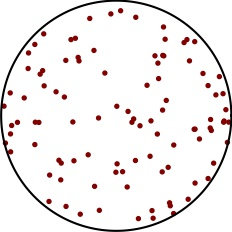
\includegraphics[width=0.065\textwidth]{images/Results/SDPS-Net/synth/lights_400_uniform}}
    \raisebox{0.12\height}{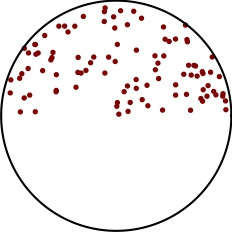
\includegraphics[width=0.065\textwidth]{images/Results/SDPS-Net/synth/lights_400_up}}
    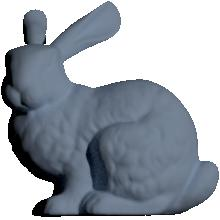
\includegraphics[width=0.081\textwidth]{images/Results/SDPS-Net/synth/samples/albedo_6_gm.jpg}
    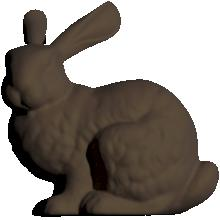
\includegraphics[width=0.081\textwidth]{images/Results/SDPS-Net/synth/samples/white-fabric_gm.jpg}
    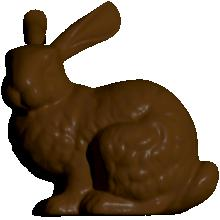
\includegraphics[width=0.081\textwidth]{images/Results/SDPS-Net/synth/samples/yellow-matte-plastic_gm.jpg}
    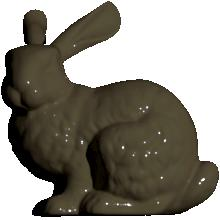
\includegraphics[width=0.075\textwidth]{images/Results/SDPS-Net/synth/samples/specular-white-phenolic_gm.jpg}
    \\
    \vspace{-0.5em}
    \makebox[0.135\textwidth]{\footnotesize (a) Light sources} 
    \makebox[0.324\textwidth]{\footnotesize (b) Examples for the four typical types of BRDFs} \\

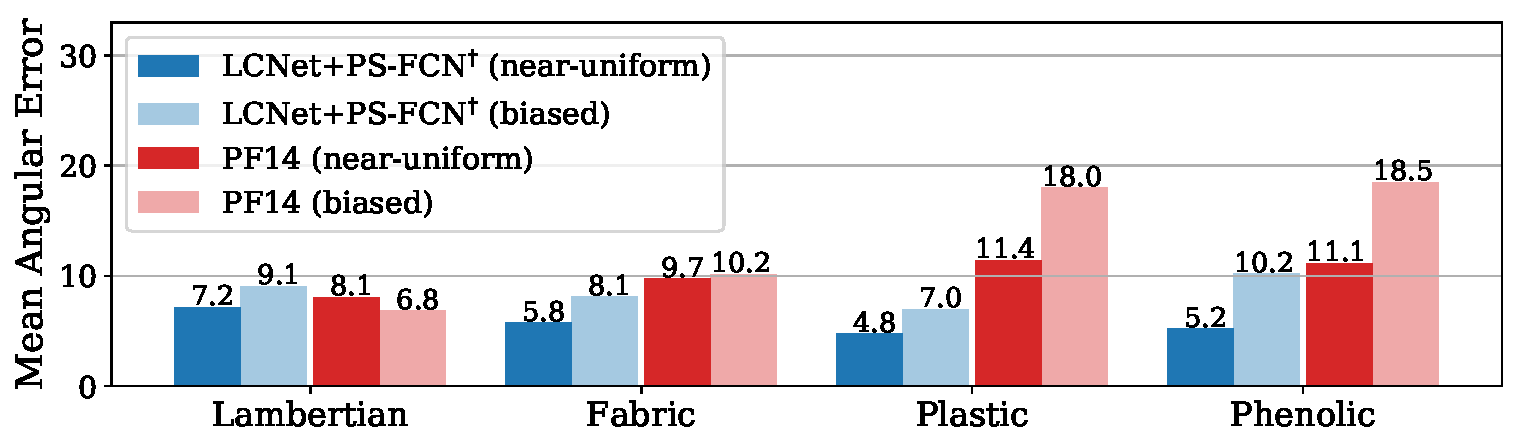
\includegraphics[width=0.49\textwidth]{images/Results/SDPS-Net/synth/compare_PF14/dir_unif}\\
\vspace{-0.7em}
\makebox[0.4\textwidth]{\footnotesize (c) Light direction estimation results} \\
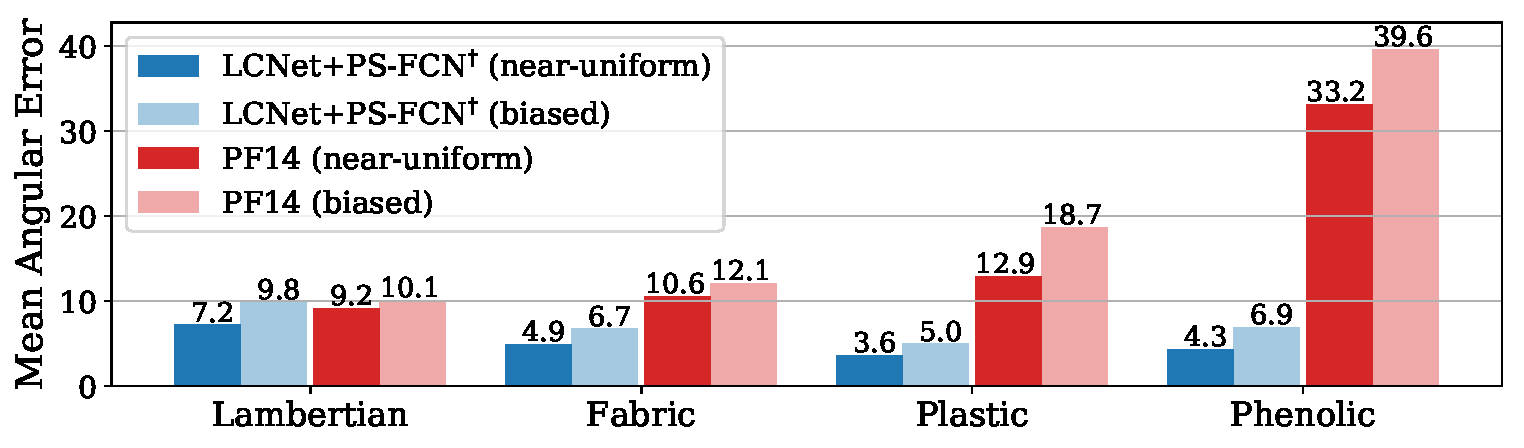
\includegraphics[width=0.49\textwidth]{images/Results/SDPS-Net/synth/compare_PF14/normal_unif}\\
\vspace{-0.7em}\makebox[0.4\textwidth]{\footnotesize (d) Surface normal estimation results}
\\
